\documentclass[]{article}
\usepackage{lmodern}
\usepackage{amssymb,amsmath}
\usepackage{ifxetex,ifluatex}
\usepackage{fixltx2e} % provides \textsubscript
\ifnum 0\ifxetex 1\fi\ifluatex 1\fi=0 % if pdftex
  \usepackage[T1]{fontenc}
  \usepackage[utf8]{inputenc}
\else % if luatex or xelatex
  \ifxetex
    \usepackage{mathspec}
  \else
    \usepackage{fontspec}
  \fi
  \defaultfontfeatures{Ligatures=TeX,Scale=MatchLowercase}
\fi
% use upquote if available, for straight quotes in verbatim environments
\IfFileExists{upquote.sty}{\usepackage{upquote}}{}
% use microtype if available
\IfFileExists{microtype.sty}{%
\usepackage{microtype}
\UseMicrotypeSet[protrusion]{basicmath} % disable protrusion for tt fonts
}{}
\usepackage[margin=1in]{geometry}
\usepackage{hyperref}
\hypersetup{unicode=true,
            pdftitle={BonusAssignment2\_Seshadri},
            pdfauthor={Sri Seshadri},
            pdfborder={0 0 0},
            breaklinks=true}
\urlstyle{same}  % don't use monospace font for urls
\usepackage{color}
\usepackage{fancyvrb}
\newcommand{\VerbBar}{|}
\newcommand{\VERB}{\Verb[commandchars=\\\{\}]}
\DefineVerbatimEnvironment{Highlighting}{Verbatim}{commandchars=\\\{\}}
% Add ',fontsize=\small' for more characters per line
\usepackage{framed}
\definecolor{shadecolor}{RGB}{248,248,248}
\newenvironment{Shaded}{\begin{snugshade}}{\end{snugshade}}
\newcommand{\KeywordTok}[1]{\textcolor[rgb]{0.13,0.29,0.53}{\textbf{#1}}}
\newcommand{\DataTypeTok}[1]{\textcolor[rgb]{0.13,0.29,0.53}{#1}}
\newcommand{\DecValTok}[1]{\textcolor[rgb]{0.00,0.00,0.81}{#1}}
\newcommand{\BaseNTok}[1]{\textcolor[rgb]{0.00,0.00,0.81}{#1}}
\newcommand{\FloatTok}[1]{\textcolor[rgb]{0.00,0.00,0.81}{#1}}
\newcommand{\ConstantTok}[1]{\textcolor[rgb]{0.00,0.00,0.00}{#1}}
\newcommand{\CharTok}[1]{\textcolor[rgb]{0.31,0.60,0.02}{#1}}
\newcommand{\SpecialCharTok}[1]{\textcolor[rgb]{0.00,0.00,0.00}{#1}}
\newcommand{\StringTok}[1]{\textcolor[rgb]{0.31,0.60,0.02}{#1}}
\newcommand{\VerbatimStringTok}[1]{\textcolor[rgb]{0.31,0.60,0.02}{#1}}
\newcommand{\SpecialStringTok}[1]{\textcolor[rgb]{0.31,0.60,0.02}{#1}}
\newcommand{\ImportTok}[1]{#1}
\newcommand{\CommentTok}[1]{\textcolor[rgb]{0.56,0.35,0.01}{\textit{#1}}}
\newcommand{\DocumentationTok}[1]{\textcolor[rgb]{0.56,0.35,0.01}{\textbf{\textit{#1}}}}
\newcommand{\AnnotationTok}[1]{\textcolor[rgb]{0.56,0.35,0.01}{\textbf{\textit{#1}}}}
\newcommand{\CommentVarTok}[1]{\textcolor[rgb]{0.56,0.35,0.01}{\textbf{\textit{#1}}}}
\newcommand{\OtherTok}[1]{\textcolor[rgb]{0.56,0.35,0.01}{#1}}
\newcommand{\FunctionTok}[1]{\textcolor[rgb]{0.00,0.00,0.00}{#1}}
\newcommand{\VariableTok}[1]{\textcolor[rgb]{0.00,0.00,0.00}{#1}}
\newcommand{\ControlFlowTok}[1]{\textcolor[rgb]{0.13,0.29,0.53}{\textbf{#1}}}
\newcommand{\OperatorTok}[1]{\textcolor[rgb]{0.81,0.36,0.00}{\textbf{#1}}}
\newcommand{\BuiltInTok}[1]{#1}
\newcommand{\ExtensionTok}[1]{#1}
\newcommand{\PreprocessorTok}[1]{\textcolor[rgb]{0.56,0.35,0.01}{\textit{#1}}}
\newcommand{\AttributeTok}[1]{\textcolor[rgb]{0.77,0.63,0.00}{#1}}
\newcommand{\RegionMarkerTok}[1]{#1}
\newcommand{\InformationTok}[1]{\textcolor[rgb]{0.56,0.35,0.01}{\textbf{\textit{#1}}}}
\newcommand{\WarningTok}[1]{\textcolor[rgb]{0.56,0.35,0.01}{\textbf{\textit{#1}}}}
\newcommand{\AlertTok}[1]{\textcolor[rgb]{0.94,0.16,0.16}{#1}}
\newcommand{\ErrorTok}[1]{\textcolor[rgb]{0.64,0.00,0.00}{\textbf{#1}}}
\newcommand{\NormalTok}[1]{#1}
\usepackage{longtable,booktabs}
\usepackage{graphicx,grffile}
\makeatletter
\def\maxwidth{\ifdim\Gin@nat@width>\linewidth\linewidth\else\Gin@nat@width\fi}
\def\maxheight{\ifdim\Gin@nat@height>\textheight\textheight\else\Gin@nat@height\fi}
\makeatother
% Scale images if necessary, so that they will not overflow the page
% margins by default, and it is still possible to overwrite the defaults
% using explicit options in \includegraphics[width, height, ...]{}
\setkeys{Gin}{width=\maxwidth,height=\maxheight,keepaspectratio}
\IfFileExists{parskip.sty}{%
\usepackage{parskip}
}{% else
\setlength{\parindent}{0pt}
\setlength{\parskip}{6pt plus 2pt minus 1pt}
}
\setlength{\emergencystretch}{3em}  % prevent overfull lines
\providecommand{\tightlist}{%
  \setlength{\itemsep}{0pt}\setlength{\parskip}{0pt}}
\setcounter{secnumdepth}{0}
% Redefines (sub)paragraphs to behave more like sections
\ifx\paragraph\undefined\else
\let\oldparagraph\paragraph
\renewcommand{\paragraph}[1]{\oldparagraph{#1}\mbox{}}
\fi
\ifx\subparagraph\undefined\else
\let\oldsubparagraph\subparagraph
\renewcommand{\subparagraph}[1]{\oldsubparagraph{#1}\mbox{}}
\fi

%%% Use protect on footnotes to avoid problems with footnotes in titles
\let\rmarkdownfootnote\footnote%
\def\footnote{\protect\rmarkdownfootnote}

%%% Change title format to be more compact
\usepackage{titling}

% Create subtitle command for use in maketitle
\newcommand{\subtitle}[1]{
  \posttitle{
    \begin{center}\large#1\end{center}
    }
}

\setlength{\droptitle}{-2em}
  \title{BonusAssignment2\_Seshadri}
  \pretitle{\vspace{\droptitle}\centering\huge}
  \posttitle{\par}
  \author{Sri Seshadri}
  \preauthor{\centering\large\emph}
  \postauthor{\par}
  \predate{\centering\large\emph}
  \postdate{\par}
  \date{3/11/2018}


\begin{document}
\maketitle

\section{Objective:}\label{objective}

Study the effect on coefficients of a model due to repeated resampling
of training and validation samples.

\section{Executive Summary}\label{executive-summary}

The coefficients of a model trained on, one time sampling of training
data, is biased. Its is necessary to train and test the model in
multiple cross validated samples to get an unbiased estimate of the
coefficients.

\section{Analysis}\label{analysis}

\subsection{Explore and Set up the data
set}\label{explore-and-set-up-the-data-set}

The structure of GermanCredit data set is explored below. It looks like
there are several binary variables that are of the type numeric. The
binary variables are converted into factors. Also there are couple of
features that have only one unique value, those featuers are removed
from the data for modeling. It'll also be useful to scale and center the
data for easier plotting of multiple coefficients in the same plot

\begin{Shaded}
\begin{Highlighting}[]
\KeywordTok{data}\NormalTok{(}\StringTok{"GermanCredit"}\NormalTok{)}
\NormalTok{skimr}\OperatorTok{::}\KeywordTok{skim}\NormalTok{(GermanCredit)}
\end{Highlighting}
\end{Shaded}

\begin{verbatim}
## Skim summary statistics
##  n obs: 1000 
##  n variables: 62 
## 
## Variable type: factor 
##  variable missing complete    n n_unique                top_counts ordered
##     Class       0     1000 1000        2 Goo: 700, Bad: 300, NA: 0   FALSE
## 
## Variable type: integer 
##                   variable missing complete    n    mean      sd  p0
##                        Age       0     1000 1000   35.55   11.38  19
##                     Amount       0     1000 1000 3271.26 2822.74 250
##                   Duration       0     1000 1000   20.9    12.06   4
##  InstallmentRatePercentage       0     1000 1000    2.97    1.12   1
##      NumberExistingCredits       0     1000 1000    1.41    0.58   1
##    NumberPeopleMaintenance       0     1000 1000    1.16    0.36   1
##          ResidenceDuration       0     1000 1000    2.85    1.1    1
##     p25 median     p75  p100     hist
##    27     33     42       75 ▇▇▆▃▂▁▁▁
##  1365.5 2319.5 3972.25 18424 ▇▃▂▁▁▁▁▁
##    12     18     24       72 ▇▅▅▃▁▁▁▁
##     2      3      4        4 ▂▁▃▁▁▂▁▇
##     1      1      2        4 ▇▁▅▁▁▁▁▁
##     1      1      1        2 ▇▁▁▁▁▁▁▂
##     2      3      4        4 ▂▁▆▁▁▃▁▇
## 
## Variable type: numeric 
##                                variable missing complete    n  mean    sd
##          CheckingAccountStatus.0.to.200       0     1000 1000 0.27  0.44 
##            CheckingAccountStatus.gt.200       0     1000 1000 0.063 0.24 
##              CheckingAccountStatus.lt.0       0     1000 1000 0.27  0.45 
##              CheckingAccountStatus.none       0     1000 1000 0.39  0.49 
##                  CreditHistory.Critical       0     1000 1000 0.29  0.46 
##                     CreditHistory.Delay       0     1000 1000 0.088 0.28 
##          CreditHistory.NoCredit.AllPaid       0     1000 1000 0.04  0.2  
##                  CreditHistory.PaidDuly       0     1000 1000 0.53  0.5  
##          CreditHistory.ThisBank.AllPaid       0     1000 1000 0.049 0.22 
##               EmploymentDuration.1.to.4       0     1000 1000 0.34  0.47 
##               EmploymentDuration.4.to.7       0     1000 1000 0.17  0.38 
##                 EmploymentDuration.gt.7       0     1000 1000 0.25  0.43 
##                 EmploymentDuration.lt.1       0     1000 1000 0.17  0.38 
##           EmploymentDuration.Unemployed       0     1000 1000 0.062 0.24 
##                           ForeignWorker       0     1000 1000 0.96  0.19 
##                         Housing.ForFree       0     1000 1000 0.11  0.31 
##                             Housing.Own       0     1000 1000 0.71  0.45 
##                            Housing.Rent       0     1000 1000 0.18  0.38 
##  Job.Management.SelfEmp.HighlyQualified       0     1000 1000 0.15  0.36 
##                     Job.SkilledEmployee       0     1000 1000 0.63  0.48 
##                 Job.UnemployedUnskilled       0     1000 1000 0.022 0.15 
##                   Job.UnskilledResident       0     1000 1000 0.2   0.4  
##      OtherDebtorsGuarantors.CoApplicant       0     1000 1000 0.041 0.2  
##        OtherDebtorsGuarantors.Guarantor       0     1000 1000 0.052 0.22 
##             OtherDebtorsGuarantors.None       0     1000 1000 0.91  0.29 
##              OtherInstallmentPlans.Bank       0     1000 1000 0.14  0.35 
##              OtherInstallmentPlans.None       0     1000 1000 0.81  0.39 
##            OtherInstallmentPlans.Stores       0     1000 1000 0.047 0.21 
##               Personal.Female.NotSingle       0     1000 1000 0.31  0.46 
##                  Personal.Female.Single       0     1000 1000 0     0    
##        Personal.Male.Divorced.Seperated       0     1000 1000 0.05  0.22 
##           Personal.Male.Married.Widowed       0     1000 1000 0.092 0.29 
##                    Personal.Male.Single       0     1000 1000 0.55  0.5  
##                       Property.CarOther       0     1000 1000 0.33  0.47 
##                      Property.Insurance       0     1000 1000 0.23  0.42 
##                     Property.RealEstate       0     1000 1000 0.28  0.45 
##                        Property.Unknown       0     1000 1000 0.15  0.36 
##                        Purpose.Business       0     1000 1000 0.097 0.3  
##               Purpose.DomesticAppliance       0     1000 1000 0.012 0.11 
##                       Purpose.Education       0     1000 1000 0.05  0.22 
##             Purpose.Furniture.Equipment       0     1000 1000 0.18  0.39 
##                          Purpose.NewCar       0     1000 1000 0.23  0.42 
##                           Purpose.Other       0     1000 1000 0.012 0.11 
##                Purpose.Radio.Television       0     1000 1000 0.28  0.45 
##                         Purpose.Repairs       0     1000 1000 0.022 0.15 
##                      Purpose.Retraining       0     1000 1000 0.009 0.094
##                         Purpose.UsedCar       0     1000 1000 0.1   0.3  
##                        Purpose.Vacation       0     1000 1000 0     0    
##          SavingsAccountBonds.100.to.500       0     1000 1000 0.1   0.3  
##         SavingsAccountBonds.500.to.1000       0     1000 1000 0.063 0.24 
##             SavingsAccountBonds.gt.1000       0     1000 1000 0.048 0.21 
##              SavingsAccountBonds.lt.100       0     1000 1000 0.6   0.49 
##             SavingsAccountBonds.Unknown       0     1000 1000 0.18  0.39 
##                               Telephone       0     1000 1000 0.6   0.49 
##  p0 p25 median p75 p100     hist
##   0   0      0   1    1 ▇▁▁▁▁▁▁▃
##   0   0      0   0    1 ▇▁▁▁▁▁▁▁
##   0   0      0   1    1 ▇▁▁▁▁▁▁▃
##   0   0      0   1    1 ▇▁▁▁▁▁▁▅
##   0   0      0   1    1 ▇▁▁▁▁▁▁▃
##   0   0      0   0    1 ▇▁▁▁▁▁▁▁
##   0   0      0   0    1 ▇▁▁▁▁▁▁▁
##   0   0      1   1    1 ▇▁▁▁▁▁▁▇
##   0   0      0   0    1 ▇▁▁▁▁▁▁▁
##   0   0      0   1    1 ▇▁▁▁▁▁▁▅
##   0   0      0   0    1 ▇▁▁▁▁▁▁▂
##   0   0      0   1    1 ▇▁▁▁▁▁▁▃
##   0   0      0   0    1 ▇▁▁▁▁▁▁▂
##   0   0      0   0    1 ▇▁▁▁▁▁▁▁
##   0   1      1   1    1 ▁▁▁▁▁▁▁▇
##   0   0      0   0    1 ▇▁▁▁▁▁▁▁
##   0   0      1   1    1 ▃▁▁▁▁▁▁▇
##   0   0      0   0    1 ▇▁▁▁▁▁▁▂
##   0   0      0   0    1 ▇▁▁▁▁▁▁▂
##   0   0      1   1    1 ▅▁▁▁▁▁▁▇
##   0   0      0   0    1 ▇▁▁▁▁▁▁▁
##   0   0      0   0    1 ▇▁▁▁▁▁▁▂
##   0   0      0   0    1 ▇▁▁▁▁▁▁▁
##   0   0      0   0    1 ▇▁▁▁▁▁▁▁
##   0   1      1   1    1 ▁▁▁▁▁▁▁▇
##   0   0      0   0    1 ▇▁▁▁▁▁▁▁
##   0   1      1   1    1 ▂▁▁▁▁▁▁▇
##   0   0      0   0    1 ▇▁▁▁▁▁▁▁
##   0   0      0   1    1 ▇▁▁▁▁▁▁▃
##   0   0      0   0    0 ▁▁▁▇▁▁▁▁
##   0   0      0   0    1 ▇▁▁▁▁▁▁▁
##   0   0      0   0    1 ▇▁▁▁▁▁▁▁
##   0   0      1   1    1 ▆▁▁▁▁▁▁▇
##   0   0      0   1    1 ▇▁▁▁▁▁▁▃
##   0   0      0   0    1 ▇▁▁▁▁▁▁▂
##   0   0      0   1    1 ▇▁▁▁▁▁▁▃
##   0   0      0   0    1 ▇▁▁▁▁▁▁▂
##   0   0      0   0    1 ▇▁▁▁▁▁▁▁
##   0   0      0   0    1 ▇▁▁▁▁▁▁▁
##   0   0      0   0    1 ▇▁▁▁▁▁▁▁
##   0   0      0   0    1 ▇▁▁▁▁▁▁▂
##   0   0      0   0    1 ▇▁▁▁▁▁▁▂
##   0   0      0   0    1 ▇▁▁▁▁▁▁▁
##   0   0      0   1    1 ▇▁▁▁▁▁▁▃
##   0   0      0   0    1 ▇▁▁▁▁▁▁▁
##   0   0      0   0    1 ▇▁▁▁▁▁▁▁
##   0   0      0   0    1 ▇▁▁▁▁▁▁▁
##   0   0      0   0    0 ▁▁▁▇▁▁▁▁
##   0   0      0   0    1 ▇▁▁▁▁▁▁▁
##   0   0      0   0    1 ▇▁▁▁▁▁▁▁
##   0   0      0   0    1 ▇▁▁▁▁▁▁▁
##   0   0      1   1    1 ▅▁▁▁▁▁▁▇
##   0   0      0   0    1 ▇▁▁▁▁▁▁▂
##   0   0      1   1    1 ▆▁▁▁▁▁▁▇
\end{verbatim}

\begin{Shaded}
\begin{Highlighting}[]
\NormalTok{integerVars <-}\StringTok{ }\NormalTok{GermanCredit  }\OperatorTok\StringTok{ }\NormalTok{dplyr}\OperatorTok{::}\KeywordTok{select_if}\NormalTok{(is.integer) }\OperatorTok\StringTok{ }\NormalTok{names}
\NormalTok{Vars <-}\StringTok{ }\KeywordTok{colnames}\NormalTok{(GermanCredit)}
\NormalTok{tobeConvertedVars <-}\StringTok{ }\NormalTok{Vars[}\OperatorTok{!}\NormalTok{Vars }\OperatorTok\StringTok{ }\NormalTok{integerVars]}

\NormalTok{GermanCredit[tobeConvertedVars] <-}\StringTok{ }\KeywordTok{lapply}\NormalTok{(GermanCredit[tobeConvertedVars], factor)}
\NormalTok{UniqueVars <-}\StringTok{ }\NormalTok{Vars[caret}\OperatorTok{::}\KeywordTok{nearZeroVar}\NormalTok{(GermanCredit,}\DataTypeTok{uniqueCut =} \DecValTok{0}\NormalTok{)]}
\NormalTok{Vars2select <-}\StringTok{ }\NormalTok{Vars[}\OperatorTok{!}\NormalTok{Vars }\OperatorTok\StringTok{ }\NormalTok{UniqueVars]}
\NormalTok{GermanCredit <-}\StringTok{ }\NormalTok{GermanCredit }\OperatorTok\StringTok{ }\NormalTok{dplyr}\OperatorTok{::}\KeywordTok{select}\NormalTok{(}\OperatorTok{!!}\NormalTok{Vars2select)}

\NormalTok{trans <-}\StringTok{ }\NormalTok{caret}\OperatorTok{::}\KeywordTok{preProcess}\NormalTok{(GermanCredit,}\DataTypeTok{center =}\NormalTok{ T, }\DataTypeTok{scale =}\NormalTok{ T)}
\NormalTok{GermanCredit <-}\StringTok{ }\KeywordTok{predict}\NormalTok{(trans, GermanCredit)}
\end{Highlighting}
\end{Shaded}

The GermanCredit data in caret package is split into training and test
in the ratio 63.2:36.8 repeatedly for 1000 times. The rsample package is
used to split the data iteratively.

The the number of rows of data for each split is verified in figure 1.

\begin{Shaded}
\begin{Highlighting}[]
\KeywordTok{set.seed}\NormalTok{(}\DecValTok{1}\NormalTok{)}
\CommentTok{# Data sampled without replacement}

\NormalTok{samples <-}\StringTok{ }\NormalTok{rsample}\OperatorTok{::}\KeywordTok{mc_cv}\NormalTok{(}\DataTypeTok{data =}\NormalTok{ GermanCredit,}\DataTypeTok{prop =} \FloatTok{0.632}\NormalTok{,}\DataTypeTok{times =} \DecValTok{1000}\NormalTok{)}

\CommentTok{# Verify the dimensions of the first of the 1000 splits}

\NormalTok{SampleVerification <-}\StringTok{ }\NormalTok{purrr}\OperatorTok{::}\KeywordTok{map_df}\NormalTok{(}\DecValTok{1}\OperatorTok{:}\DecValTok{1000}\NormalTok{,}\DataTypeTok{.f =} \ControlFlowTok{function}\NormalTok{(x) }\KeywordTok{data.frame}\NormalTok{(}\DataTypeTok{ResampleId =}\NormalTok{ x,}\DataTypeTok{TrainRows =} \KeywordTok{nrow}\NormalTok{(}\KeywordTok{analysis}\NormalTok{(samples}\OperatorTok{$}\NormalTok{splits[[x]])), }\DataTypeTok{TestRows =} \KeywordTok{nrow}\NormalTok{(}\KeywordTok{assessment}\NormalTok{(samples}\OperatorTok{$}\NormalTok{splits[[x]]))) )}

\NormalTok{lattice}\OperatorTok{::}\KeywordTok{xyplot}\NormalTok{(TrainRows }\OperatorTok{+}\StringTok{ }\NormalTok{TestRows }\OperatorTok{~}\StringTok{ }\NormalTok{ResampleId,}\DataTypeTok{data =}\NormalTok{ SampleVerification,}\DataTypeTok{ylab =} \StringTok{"Rows of data"}\NormalTok{,}\DataTypeTok{auto.key=}\KeywordTok{list}\NormalTok{(}\DataTypeTok{space=}\StringTok{"bottom"}\NormalTok{, }\DataTypeTok{columns=}\DecValTok{4}\NormalTok{, }\DataTypeTok{cex.title=}\DecValTok{1}\NormalTok{,}\DataTypeTok{lines=}\OtherTok{TRUE}\NormalTok{, }\DataTypeTok{points=}\OtherTok{FALSE}\NormalTok{, }\DataTypeTok{box =}\NormalTok{ T))}
\end{Highlighting}
\end{Shaded}

\begin{figure}
\centering
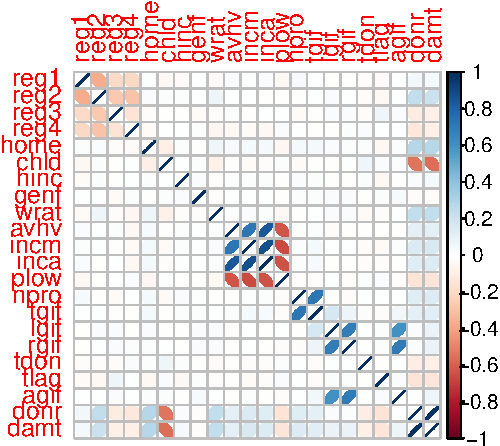
\includegraphics{BonusAssignment2_files/figure-latex/unnamed-chunk-2-1.pdf}
\caption{Verify split}
\end{figure}

\subsection{Linear model fits and
evaluation.}\label{linear-model-fits-and-evaluation.}

Linear model is fit on the training sets and the model is evaluated on
the test sets for each of the 1000 train-test samples. Those variables
that have only one unique value are removed as predictors.

\begin{Shaded}
\begin{Highlighting}[]
\CommentTok{# Function to get model stats}
\NormalTok{ModelSummaries <-}\StringTok{ }\ControlFlowTok{function}\NormalTok{(split)\{}
  \CommentTok{# get the train and test sets from the split}
\NormalTok{  Train <-}\StringTok{ }\NormalTok{rsample}\OperatorTok{::}\KeywordTok{analysis}\NormalTok{(split}\OperatorTok{$}\NormalTok{splits[[}\DecValTok{1}\NormalTok{]])}
\NormalTok{  Test <-}\StringTok{ }\NormalTok{rsample}\OperatorTok{::}\KeywordTok{assessment}\NormalTok{(split}\OperatorTok{$}\NormalTok{splits[[}\DecValTok{1}\NormalTok{]])}
\NormalTok{  Vars <-}\StringTok{ }\KeywordTok{colnames}\NormalTok{(Train)}
  \CommentTok{# get variables that have only one unique value and remove them}
\NormalTok{  UniqueVars <-}\StringTok{ }\NormalTok{caret}\OperatorTok{::}\KeywordTok{nearZeroVar}\NormalTok{(Train,}\DataTypeTok{uniqueCut =} \DecValTok{0}\NormalTok{)}
  \ControlFlowTok{if}\NormalTok{(}\KeywordTok{length}\NormalTok{(UniqueVars) }\OperatorTok{>}\StringTok{ }\DecValTok{0}\NormalTok{)\{}
\NormalTok{    Train <-}\StringTok{ }\NormalTok{Train[,UniqueVars}\OperatorTok{*-}\DecValTok{1}\NormalTok{]}
\NormalTok{    Test <-}\StringTok{ }\NormalTok{Test[,UniqueVars}\OperatorTok{*-}\DecValTok{1}\NormalTok{]}
\NormalTok{  \}}
  
  
  \CommentTok{# linear model fit}
\NormalTok{  lm.fit <-}\StringTok{ }\KeywordTok{lm}\NormalTok{(Amount }\OperatorTok{~}\StringTok{ }\NormalTok{., }\DataTypeTok{data =}\NormalTok{ Train)}
\NormalTok{  coefs <-}\StringTok{ }\KeywordTok{coefficients}\NormalTok{(lm.fit)}
\NormalTok{  AdjR2.Train <-}\StringTok{ }\KeywordTok{summary}\NormalTok{(lm.fit)}\OperatorTok{$}\NormalTok{adj.r.squared}
\NormalTok{  yPred <-}\StringTok{ }\KeywordTok{predict}\NormalTok{(lm.fit,}\DataTypeTok{newdata =}\NormalTok{ Test)}
\NormalTok{  R2.test <-}\StringTok{ }\KeywordTok{cor}\NormalTok{(yPred,Test}\OperatorTok{$}\NormalTok{Amount)}\OperatorTok{^}\DecValTok{2}
  \KeywordTok{return}\NormalTok{(}\KeywordTok{list}\NormalTok{(}\DataTypeTok{Betas =}\NormalTok{ coefs,}\DataTypeTok{Train.R2 =}\NormalTok{ AdjR2.Train, }\DataTypeTok{Test.R2 =}\NormalTok{ R2.test))}
\NormalTok{\}}

\NormalTok{ModelStats <-}\StringTok{ }\NormalTok{purrr}\OperatorTok{::}\KeywordTok{map}\NormalTok{(}\DecValTok{1}\OperatorTok{:}\DecValTok{1000}\NormalTok{,}\ControlFlowTok{function}\NormalTok{(x) }\KeywordTok{ModelSummaries}\NormalTok{(samples[x,]))}

\CommentTok{# Check if named vectors of Beta coefficients are the same for all the 1000 splits}
\NormalTok{lengthVer <-}\StringTok{ }\KeywordTok{sapply}\NormalTok{(}\DecValTok{1}\OperatorTok{:}\DecValTok{1000}\NormalTok{,}\ControlFlowTok{function}\NormalTok{(x) }\KeywordTok{names}\NormalTok{(ModelStats[[x]]}\OperatorTok{$}\NormalTok{Betas))}
\NormalTok{test2 <-}\StringTok{ }\KeywordTok{sapply}\NormalTok{(}\DecValTok{1}\OperatorTok{:}\DecValTok{60}\NormalTok{, }\ControlFlowTok{function}\NormalTok{(x) \{}\KeywordTok{length}\NormalTok{(}\KeywordTok{unique}\NormalTok{(lengthVer[x,]))\})}
\CommentTok{#plot(test2)}

\CommentTok{# Retrieve Beta coefficents as dataframe}

\NormalTok{df.coef <-}\StringTok{ }\KeywordTok{sapply}\NormalTok{(}\DecValTok{1}\OperatorTok{:}\DecValTok{1000}\NormalTok{, }\ControlFlowTok{function}\NormalTok{(x)\{ModelStats[[x]]}\OperatorTok{$}\NormalTok{Betas\})}
\NormalTok{df.coef <-}\StringTok{ }\KeywordTok{t}\NormalTok{(df.coef)}

\NormalTok{Rsquared <-}\StringTok{ }\KeywordTok{data.frame}\NormalTok{(}\DataTypeTok{Train =}\NormalTok{ train <-}\StringTok{ }\KeywordTok{sapply}\NormalTok{(}\DecValTok{1}\OperatorTok{:}\DecValTok{1000}\NormalTok{, }\ControlFlowTok{function}\NormalTok{(x)\{ModelStats[[x]]}\OperatorTok{$}\NormalTok{Train.R2\}),}
                       \DataTypeTok{Test =} \KeywordTok{sapply}\NormalTok{(}\DecValTok{1}\OperatorTok{:}\DecValTok{1000}\NormalTok{, }\ControlFlowTok{function}\NormalTok{(x)\{ModelStats[[x]]}\OperatorTok{$}\NormalTok{Test.R2\}))}

\NormalTok{Rsquared <-}\StringTok{ }\NormalTok{Rsquared }\OperatorTok\StringTok{ }\KeywordTok{mutate}\NormalTok{(}\DataTypeTok{PercFall =}\NormalTok{ (Train }\OperatorTok{-}\StringTok{ }\NormalTok{Test)}\OperatorTok{/}\NormalTok{Train)}
\end{Highlighting}
\end{Shaded}

Figure 2 shows the scaled coefficients of the predictors.

\begin{Shaded}
\begin{Highlighting}[]
\NormalTok{df.coef <-}\StringTok{ }\KeywordTok{data.frame}\NormalTok{(df.coef)}
\NormalTok{df.coef.plotdf <-}\StringTok{ }\NormalTok{tidyr}\OperatorTok{::}\KeywordTok{gather}\NormalTok{(df.coef)}
\KeywordTok{ggplot}\NormalTok{(}\DataTypeTok{data =}\NormalTok{ df.coef.plotdf, }\DataTypeTok{mapping =} \KeywordTok{aes}\NormalTok{(}\DataTypeTok{x=}\NormalTok{value)) }\OperatorTok{+}\StringTok{ }\KeywordTok{geom_histogram}\NormalTok{() }\OperatorTok{+}\StringTok{ }\KeywordTok{facet_wrap}\NormalTok{(}\OperatorTok{~}\NormalTok{key, }\DataTypeTok{scales =} \StringTok{'free_x'}\NormalTok{)}
\end{Highlighting}
\end{Shaded}

\begin{verbatim}
## `stat_bin()` using `bins = 30`. Pick better value with `binwidth`.
\end{verbatim}

\begin{verbatim}
## Warning: Removed 11000 rows containing non-finite values (stat_bin).
\end{verbatim}

\begin{figure}
\centering
\includegraphics{BonusAssignment2_files/figure-latex/unnamed-chunk-4-1.pdf}
\caption{Scaled Coefficients plot}
\end{figure}

Figure 3 shows the distribution of R-Squared of Training and Test data
and as well the \% fall in R-Squared from training to test.

It can be seen that the \% Fall in R Squared is within a range of -20\%
to 30\%.

\begin{Shaded}
\begin{Highlighting}[]
\KeywordTok{par}\NormalTok{(}\DataTypeTok{mfrow=}\KeywordTok{c}\NormalTok{(}\DecValTok{1}\NormalTok{,}\DecValTok{3}\NormalTok{))}
\KeywordTok{hist}\NormalTok{(Rsquared}\OperatorTok{$}\NormalTok{Train,}\DataTypeTok{xlab =} \StringTok{"RSquared Training"}\NormalTok{, }\DataTypeTok{main=}\StringTok{""}\NormalTok{)}
\KeywordTok{hist}\NormalTok{(Rsquared}\OperatorTok{$}\NormalTok{Test,}\DataTypeTok{xlab =} \StringTok{"RSquared Test"}\NormalTok{, }\DataTypeTok{main=}\StringTok{""}\NormalTok{)}
\KeywordTok{hist}\NormalTok{(Rsquared}\OperatorTok{$}\NormalTok{PercFall, }\DataTypeTok{xlab =} \StringTok{"% Fall in RSquared from Train to Test"}\NormalTok{, }\DataTypeTok{main=}\StringTok{""}\NormalTok{)}
\end{Highlighting}
\end{Shaded}

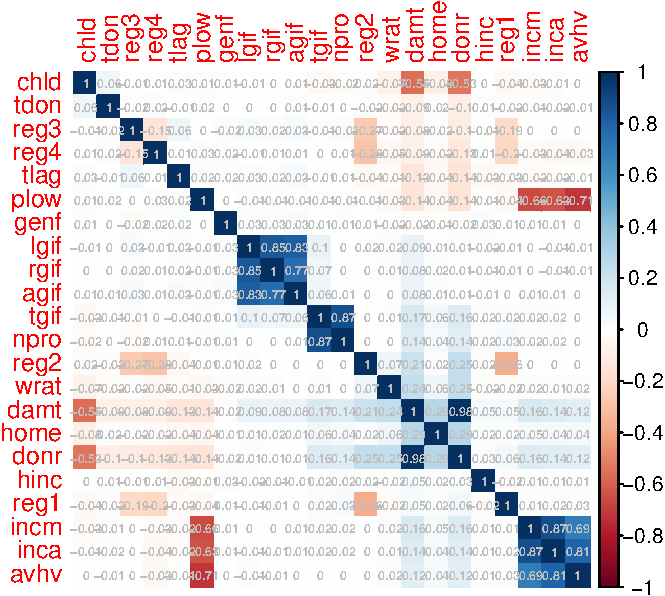
\includegraphics{BonusAssignment2_files/figure-latex/unnamed-chunk-5-1.pdf}

\begin{Shaded}
\begin{Highlighting}[]
\KeywordTok{library}\NormalTok{(Rmisc)}
\end{Highlighting}
\end{Shaded}

\begin{verbatim}
## Loading required package: plyr
\end{verbatim}

\begin{verbatim}
## -------------------------------------------------------------------------
\end{verbatim}

\begin{verbatim}
## You have loaded plyr after dplyr - this is likely to cause problems.
## If you need functions from both plyr and dplyr, please load plyr first, then dplyr:
## library(plyr); library(dplyr)
\end{verbatim}

\begin{verbatim}
## -------------------------------------------------------------------------
\end{verbatim}

\begin{verbatim}
## 
## Attaching package: 'plyr'
\end{verbatim}

\begin{verbatim}
## The following objects are masked from 'package:dplyr':
## 
##     arrange, count, desc, failwith, id, mutate, rename, summarise,
##     summarize
\end{verbatim}

\begin{Shaded}
\begin{Highlighting}[]
\NormalTok{Stats <-}\StringTok{ }\KeywordTok{data.frame}\NormalTok{(}\KeywordTok{t}\NormalTok{(}\KeywordTok{sapply}\NormalTok{(}\DecValTok{1}\OperatorTok{:}\DecValTok{60}\NormalTok{, }\ControlFlowTok{function}\NormalTok{(x)\{}\KeywordTok{CI}\NormalTok{(df.coef[,x])\}))) }\OperatorTok\StringTok{ }\NormalTok{dplyr}\OperatorTok{::}\KeywordTok{mutate}\NormalTok{(}\DataTypeTok{Predictor =} \KeywordTok{colnames}\NormalTok{(df.coef)) }\OperatorTok\StringTok{ }
\StringTok{  }\NormalTok{dplyr}\OperatorTok{::}\KeywordTok{select}\NormalTok{(Predictor,lower,mean,upper)}

\NormalTok{trainSamples <-}\StringTok{ }\KeywordTok{sample}\NormalTok{(}\DecValTok{1000}\NormalTok{,}\DecValTok{632}\NormalTok{)}
\CommentTok{#nearZeroVar(GermanCredit[train,],uniqueCut = 0)}
\NormalTok{lmfit.once <-}\StringTok{ }\KeywordTok{lm}\NormalTok{(Amount }\OperatorTok{~}\StringTok{ }\NormalTok{., }\DataTypeTok{data =}\NormalTok{ GermanCredit[trainSamples,])}
\NormalTok{coefs.omce <-}\StringTok{ }\KeywordTok{coef}\NormalTok{(lmfit.once)}
\NormalTok{Stats <-}\StringTok{ }\NormalTok{Stats }\OperatorTok\StringTok{ }\NormalTok{dplyr}\OperatorTok{::}\KeywordTok{mutate}\NormalTok{(}\DataTypeTok{OneTimeSplitCoef =}\NormalTok{ coefs.omce, }\DataTypeTok{WithinCI =} \KeywordTok{if_else}\NormalTok{(coefs.omce }\OperatorTok{>=}\StringTok{ }\NormalTok{lower }\OperatorTok{&}\StringTok{ }\NormalTok{coefs.omce }\OperatorTok{<=}\StringTok{ }\NormalTok{upper,}\StringTok{"Within"}\NormalTok{,}\StringTok{"Outside"}\NormalTok{))}

\NormalTok{knitr}\OperatorTok{::}\KeywordTok{kable}\NormalTok{(Stats, }\DataTypeTok{caption =} \StringTok{"Comparison of single coefficient to averge of 1000 fits"}\NormalTok{)}
\end{Highlighting}
\end{Shaded}

\begin{longtable}[]{@{}lrrrrl@{}}
\caption{Comparison of single coefficient to averge of 1000
fits}\tabularnewline
\toprule
Predictor & lower & mean & upper & OneTimeSplitCoef &
WithinCI\tabularnewline
\midrule
\endfirsthead
\toprule
Predictor & lower & mean & upper & OneTimeSplitCoef &
WithinCI\tabularnewline
\midrule
\endhead
X.Intercept. & 1.3610675 & 1.3883982 & 1.4157290 & 1.0076342 &
Outside\tabularnewline
Duration & 0.5293622 & 0.5309347 & 0.5325073 & 0.4872938 &
Outside\tabularnewline
InstallmentRatePercentage & -0.3165723 & -0.3153660 & -0.3141596 &
-0.3045645 & Outside\tabularnewline
ResidenceDuration & -0.0205579 & -0.0193493 & -0.0181408 & -0.0012570 &
Outside\tabularnewline
Age & 0.0255229 & 0.0268692 & 0.0282155 & 0.0187196 &
Outside\tabularnewline
NumberExistingCredits & 0.0110226 & 0.0123172 & 0.0136119 & 0.0197262 &
Outside\tabularnewline
NumberPeopleMaintenance & -0.0275179 & -0.0264781 & -0.0254383 &
-0.0548516 & Outside\tabularnewline
Telephone1 & -0.1750750 & -0.1726407 & -0.1702064 & -0.1299213 &
Outside\tabularnewline
ForeignWorker1 & -0.1040195 & -0.0986412 & -0.0932629 & -0.0122258 &
Outside\tabularnewline
ClassGood & -0.1336153 & -0.1305027 & -0.1273901 & -0.0976242 &
Outside\tabularnewline
CheckingAccountStatus.lt.01 & -0.0748525 & -0.0719788 & -0.0691051 &
0.0200919 & Outside\tabularnewline
CheckingAccountStatus.0.to.2001 & 0.0447519 & 0.0473957 & 0.0500395 &
0.1019934 & Outside\tabularnewline
CheckingAccountStatus.gt.2001 & -0.2290817 & -0.2258868 & -0.2226919 &
-0.2629068 & Outside\tabularnewline
CheckingAccountStatus.none1 & NA & NA & NA & NA & NA\tabularnewline
CreditHistory.NoCredit.AllPaid1 & 0.2535960 & 0.2606260 & 0.2676560 &
0.0358525 & Outside\tabularnewline
CreditHistory.ThisBank.AllPaid1 & -0.0628903 & -0.0569821 & -0.0510739 &
-0.0489794 & Outside\tabularnewline
CreditHistory.PaidDuly1 & -0.0244654 & -0.0217219 & -0.0189783 &
0.0864416 & Outside\tabularnewline
CreditHistory.Delay1 & 0.0202810 & 0.0249907 & 0.0297005 & 0.1181631 &
Outside\tabularnewline
CreditHistory.Critical1 & NA & NA & NA & NA & NA\tabularnewline
Purpose.NewCar1 & -0.6661461 & -0.6420297 & -0.6179133 & -0.6664775 &
Outside\tabularnewline
Purpose.UsedCar1 & -0.4125948 & -0.3884939 & -0.3643930 & -0.2902017 &
Outside\tabularnewline
Purpose.Furniture.Equipment1 & -0.6794603 & -0.6552790 & -0.6310976 &
-0.7004469 & Outside\tabularnewline
Purpose.Radio.Television1 & -0.7600349 & -0.7360964 & -0.7121579 &
-0.7989457 & Outside\tabularnewline
Purpose.DomesticAppliance1 & -0.9098339 & -0.8848707 & -0.8599074 &
-0.9329383 & Outside\tabularnewline
Purpose.Repairs1 & -0.6422480 & -0.6173233 & -0.5923987 & -0.8524553 &
Outside\tabularnewline
Purpose.Education1 & -0.7181040 & -0.6938231 & -0.6695422 & -0.6701855 &
Within\tabularnewline
Purpose.Retraining1 & -0.7903655 & -0.7640032 & -0.7376408 & -1.0415600
& Outside\tabularnewline
Purpose.Business1 & -0.7283467 & -0.7041555 & -0.6799643 & -0.7783022 &
Outside\tabularnewline
Purpose.Other1 & NA & NA & NA & NA & NA\tabularnewline
SavingsAccountBonds.lt.1001 & -0.1316095 & -0.1284673 & -0.1253251 &
-0.0652545 & Outside\tabularnewline
SavingsAccountBonds.100.to.5001 & -0.2103486 & -0.2063924 & -0.2024363 &
-0.2305228 & Outside\tabularnewline
SavingsAccountBonds.500.to.10001 & -0.2353459 & -0.2309910 & -0.2266360
& -0.1632795 & Outside\tabularnewline
SavingsAccountBonds.gt.10001 & -0.1345730 & -0.1303231 & -0.1260732 &
-0.0734524 & Outside\tabularnewline
SavingsAccountBonds.Unknown1 & NA & NA & NA & NA & NA\tabularnewline
EmploymentDuration.lt.11 & 0.0320726 & 0.0387220 & 0.0453713 & 0.0887161
& Outside\tabularnewline
EmploymentDuration.1.to.41 & 0.0139163 & 0.0206067 & 0.0272970 &
0.0880706 & Outside\tabularnewline
EmploymentDuration.4.to.71 & 0.0470244 & 0.0540457 & 0.0610669 &
0.2346389 & Outside\tabularnewline
EmploymentDuration.gt.71 & -0.0595789 & -0.0527727 & -0.0459665 &
0.0612719 & Outside\tabularnewline
EmploymentDuration.Unemployed1 & NA & NA & NA & NA & NA\tabularnewline
Personal.Male.Divorced.Seperated1 & 0.1474485 & 0.1528003 & 0.1581521 &
0.2172886 & Outside\tabularnewline
Personal.Female.NotSingle1 & 0.0909682 & 0.0938667 & 0.0967652 &
0.0448338 & Outside\tabularnewline
Personal.Male.Single1 & 0.2588820 & 0.2619492 & 0.2650164 & 0.2710714 &
Outside\tabularnewline
Personal.Male.Married.Widowed1 & NA & NA & NA & NA & NA\tabularnewline
OtherDebtorsGuarantors.None1 & 0.0228669 & 0.0267009 & 0.0305350 &
0.0014942 & Outside\tabularnewline
OtherDebtorsGuarantors.CoApplicant1 & 0.2226994 & 0.2291624 & 0.2356255
& 0.3369058 & Outside\tabularnewline
OtherDebtorsGuarantors.Guarantor1 & NA & NA & NA & NA &
NA\tabularnewline
Property.RealEstate1 & -0.2927526 & -0.2862939 & -0.2798351 & -0.2358026
& Outside\tabularnewline
Property.Insurance1 & -0.2098111 & -0.2031548 & -0.1964984 & -0.1448284
& Outside\tabularnewline
Property.CarOther1 & -0.2010101 & -0.1944734 & -0.1879366 & -0.0916335 &
Outside\tabularnewline
Property.Unknown1 & NA & NA & NA & NA & NA\tabularnewline
OtherInstallmentPlans.Bank1 & -0.0624438 & -0.0592244 & -0.0560049 &
-0.0850008 & Outside\tabularnewline
OtherInstallmentPlans.Stores1 & -0.0334157 & -0.0275384 & -0.0216611 &
-0.0317454 & Within\tabularnewline
OtherInstallmentPlans.None1 & NA & NA & NA & NA & NA\tabularnewline
Housing.Rent1 & 0.0666029 & 0.0746474 & 0.0826919 & 0.0461640 &
Outside\tabularnewline
Housing.Own1 & 0.0369494 & 0.0448396 & 0.0527299 & 0.0792720 &
Outside\tabularnewline
Housing.ForFree1 & NA & NA & NA & NA & NA\tabularnewline
Job.UnemployedUnskilled1 & -0.5949737 & -0.5818403 & -0.5687068 &
-0.3422740 & Outside\tabularnewline
Job.UnskilledResident1 & -0.4269291 & -0.4219083 & -0.4168875 &
-0.5008756 & Outside\tabularnewline
Job.SkilledEmployee1 & -0.4456681 & -0.4411288 & -0.4365895 & -0.4424048
& Within\tabularnewline
Job.Management.SelfEmp.HighlyQualified1 & NA & NA & NA & NA &
NA\tabularnewline
\bottomrule
\end{longtable}

\begin{Shaded}
\begin{Highlighting}[]
\KeywordTok{table}\NormalTok{(Stats}\OperatorTok{$}\NormalTok{WithinCI)}
\end{Highlighting}
\end{Shaded}

\begin{verbatim}
## 
## Outside  Within 
##      46       3
\end{verbatim}

\section{Conclusion}\label{conclusion}

It is seen that 47 of 49 coeffiicents of the one time split model are
outside of the confidence interval. This is due to the 1000 samples of
each coefficients making the confidence intterval tight. The one time
sample coefficient is a biased estimate, whereas the avergae of 1000
samples of each coefficent is unbiased.


\end{document}
